% !TEX TS-program = xelatex
% !TEX encoding = UTF-8 Unicode
% !Mode:: "TeX:UTF-8"

\documentclass{resume}
\usepackage{zh_CN-Adobefonts_external} % Simplified Chinese Support using external fonts (./fonts/zh_CN-Adobe/)
%\usepackage{zh_CN-Adobefonts_internal} % Simplified Chinese Support using system fonts
\usepackage{linespacing_fix} % disable extra space before next section
\usepackage{cite}
\usepackage{graphicx}
\usepackage{geometry}
\usepackage{multicol}
\usepackage{tabularray}
\usepackage{enumitem}


\geometry{a4paper,left=1.5cm,right=1.5cm,top=1.2cm,bottom=1.2cm} % 修改页边距,使得内容在一页范围内
\begin{document}
\pagenumbering{gobble} % suppress displaying page number




% {E-mail}{mobilephone}{homepage}
% be careful of _ in emaill address

\iffalse 
\name{陈冠斌}
\contactInfo{(+86)15682871716}{1249591860@qq.com}{C++开发}{}
\contactInfo{GitHub \textit{github.com/congmingyige}}{Blog \textit{cnblogs.com/cmyg}}{}{}
\fi

\begin{minipage}[t]{0.78\textwidth} % 调整minipage多个0.78/0.15/0.07,0.8/0.2的大小,调整图片width的大小,调整\vspace移动大小
	\centering
	\name{\Huge 陈冠斌} % 增大字体
	\vspace{0.5em} % 调整名字和联系信息的间距
	\contactInfo{(+86)15682871716}{1249591860@qq.com}{OI编程教练}{}
	\contactInfo{GitHub \textit{github.com/congmingyige}}{Blog \textit{cnblogs.com/cmyg}}{}{}
\end{minipage}%
\begin{minipage}[t]{0.15\textwidth}
	\vspace{-2.4em} % 通过负值将图片向上移动 % 调整数值:\vspace
	\begin{flushright}
		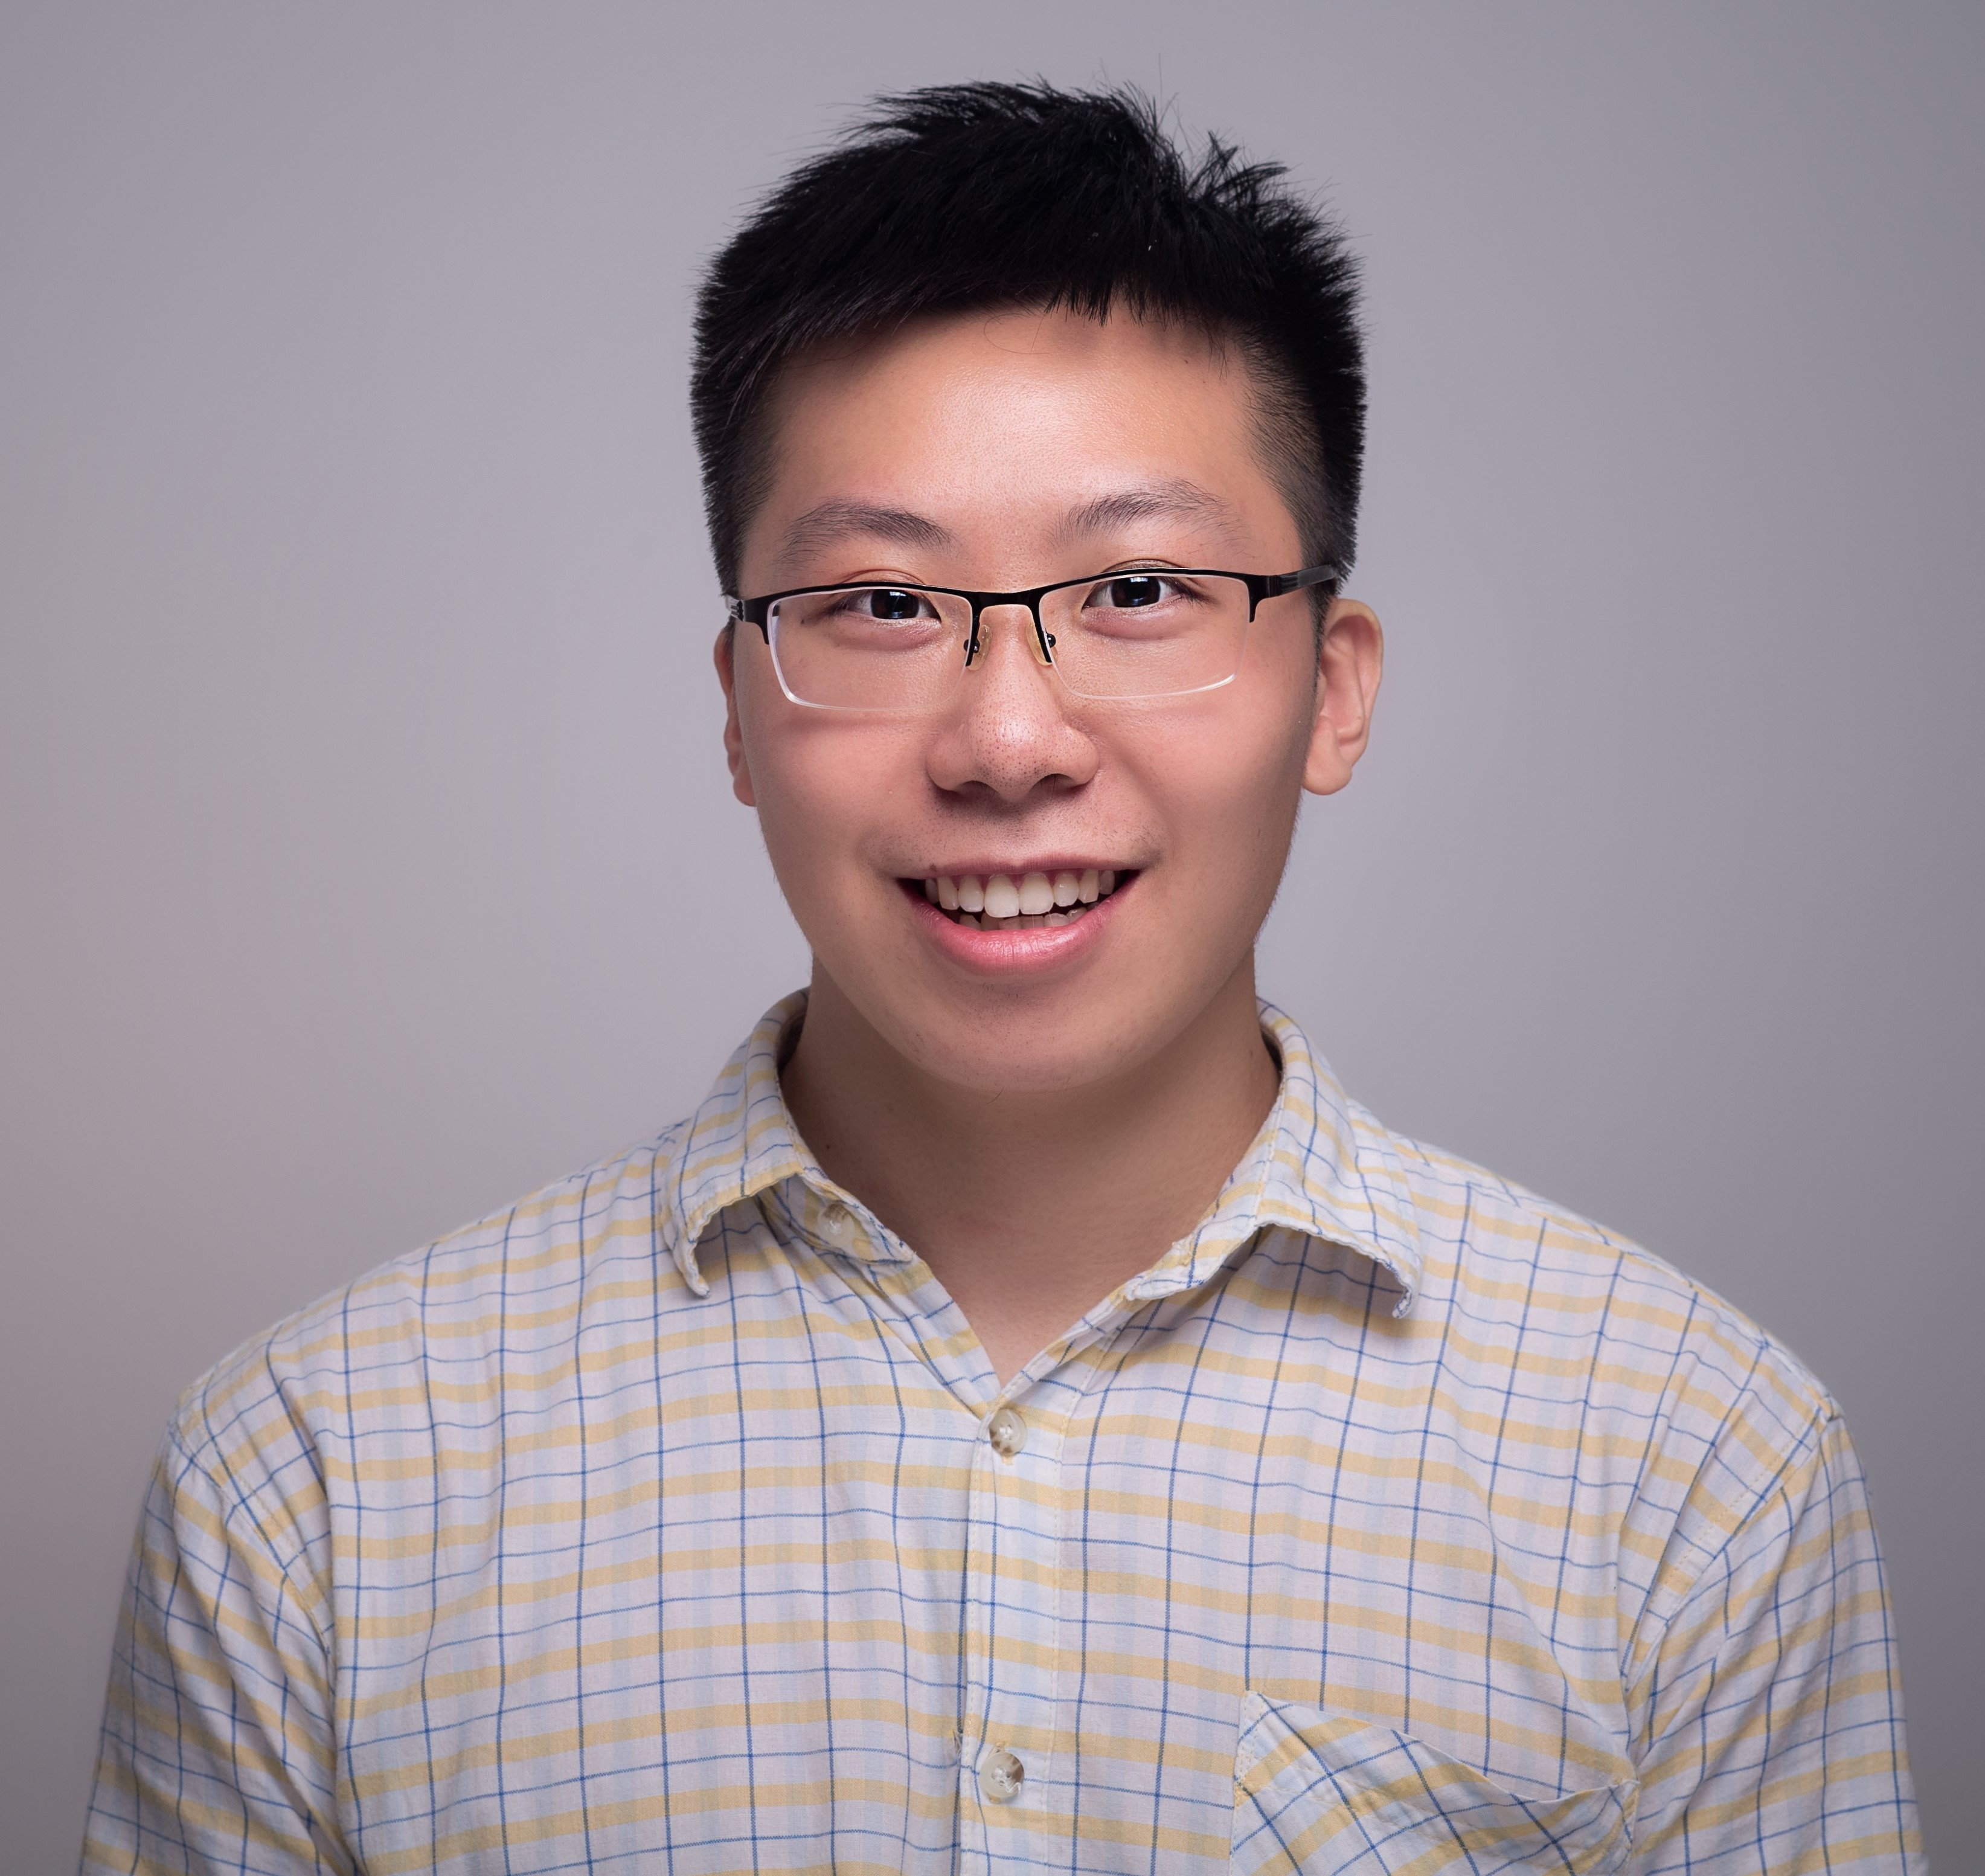
\includegraphics[width=1\textwidth]{cgb.jpg} % 调整图片大小以适配文字高度
	\end{flushright}
\end{minipage}
\begin{minipage}[t]{0.07\textwidth}
\end{minipage}


% $\photo[64pt]{./cgb_3712_3712.jpg}


% {E-mail}{mobilephone}
% keep the last empty braces!
%\contactInfo{xxx@yuanbin.me}{(+86) 131-221-87xxx}{}

\section{个人总结}
擅长\textbf{C++}语言,对\textbf{常用数据结构和算法}具有敏锐的直觉与兴趣。曾获得\textbf{ ACM-ICPC 银奖}、\textbf{高教杯数学建模全国二等奖}以及\textbf{本科国家奖学金}。

% \section{\faGraduationCap\ 教育背景}
\section{教育背景}

\datedsubsection{\textbf{兰州大学},\textbf{计算机科学与技术},\textit{学士}}{2015.9 - 2019.6}
学业成绩排名2/69(前5\%),国家奖学金,优秀学生一等奖学金,学生标兵,兰州大学优秀毕业生
\datedsubsection{\textbf{华中科技大学},\textbf{计算机科学与技术},\textit{在读硕士研究生}}{2019.9 - 2025.6}
学业成绩排名前50\%,一等学业奖学金,共青团先进个人,预计2025年6月毕业。保送直博,直博转硕


% \begin{onehalfspacing}
% \end{onehalfspacing}

% \datedsubsection{\textbf{DID-ACTE} 荷兰莱顿}{2015年}
% \role{本科毕业设计}{LIACS 交换生}
% 利用结巴分词对中国古文进行分词与词性标注,用已有领域知识训练形成 classifier 并对结果进行调优
% \begin{onehalfspacing}
% \begin{itemize}
%   \item 利用结巴分词对中国古文进行分词与词性标注
%   \item 利用已有领域知识训练形成 classifier, 并用分词结果进行测试反馈
%   \item 尝试不同规则,对 classifier 进行调优
% \end{itemize}
% \end{onehalfspacing}

\section{竞赛获奖/项目作品}
% increase linespacing [parsep=0.5ex]
\begin{itemize}[parsep=0.2ex]
%   \item LeetCodeOJ Solutions, \textit{https://github.com/hijiangtao/LeetCodeOJ}
  \item \textbf{ACM银奖}(2018亚洲区域赛焦作银奖、2018亚洲区域赛青岛银奖)
  \item \textbf{高教社杯数学建模本科组全国二等奖}
  \item 中国高校计算机大赛-团体程序设计天梯赛(CCCC)甘肃赛"珠峰登顶"组特等奖
  \item CSP计算机认证多次 $\geq$ 300分
  \item NOIP普及组全国一等奖(广东省第7) \& NOIP提高组到达除广东省以外其它省份的一等奖分数线
  \item 初中数学竞赛全国一等奖(初二时与初三同台竞技获得)
  
\end{itemize}


% \section{\faCogs\ IT 技能}
\section{技术能力}
% increase linespacing [parsep=0.5ex]
\begin{itemize}[parsep=0.2ex]
	\item \textbf{编程语言和工具}: 熟练掌握 C++ / 掌握 Python / JavaScript / Git / CET-6
	\item \textbf{专业技能}:了解 Linux / 计算机网络 / 操作系统 / SQL
\end{itemize}

% \end{itemize}

\section{项目经历}
\datedsubsection{\textbf{基于Swin Transformer方法的脑损伤全脑血管的分割和重建}}{}
\begin{itemize}
	\item \textbf{问题和描述}:三维图像血管分割和重建问题。血管存在二维和三维上的边缘断裂,信号不连续,干扰信号等问题。数据为三维数据,数据量极大,而且血管直径跨越多个数量级且结构复杂。
	\item \textbf{3D特征提取网络的构建}:针对二维和三维信号不连续问题,学习图像中的上下文相关性,实现包含连通性和拓扑结构的完整分割。
	\item \textbf{多尺度的特征提取}:通过层次化构建提取多尺度特征。其滑动窗口的多头自注意模块 (SW-MSA) 促进了窗口间的信息交互,并大幅降低计算量,解决了超大三维图像数据集分割速度慢的问题。
	\item \textbf{运行环境}:网络使用 Pytorch 实现。实验在配备 8 个 NVIDIA Tesla V100 GPU 32GB 的服务器上并行训练。
	\item \textbf{评估指标}:采用Accuracy、Precision、Recall、F1、clDice等参数进行评估。
\end{itemize}

\datedsubsection{\textbf{兰州大学程序设计竞赛等多项编程比赛的组织与出题}}{}
\begin{itemize}
	\item \textbf{团队协作}:通过团队交流提升题目设计的质量,进行交叉验题,确保项目严格按照截止日期推进。
	\item \textbf{规范化流程}:利用Polygon平台进行出题,设计极限数据,不同解法在比赛运行平台进行多重测试。
	\item \textbf{创新性和行业贡献}:挖掘新的问题和算法场景,探索不同数据范围和约束下的解法,致力于做具有成就感和行业价值的事情。
	\item \textbf{个人成长}:在经历500多道题的经典算法题目学习基础上,共参与出题20余道,参与验题30余道,对动态规划、图论、搜索、树等数据结构和算法有更深了解,精通常用的计算机数据结构和算法。
\end{itemize}

% \section{\faHeartO\ 项目/作品摘要}
% \section{项目/作品摘要}
% \datedline{\textit{An Integrated Version of Security Monitor Vis System}, https://hijiangtao.github.io/ss-vis-component/ }{}
% \datedline{\textit{Dark-Tech}, https://github.com/hijiangtao/dark-tech/ }{}
% \datedline{\textit{融合社交网络数据挖掘的电视节目可视化分析系统}, https://hijiangtao.github.io/variety-show-hot-spot-vis/}{}
% \datedline{\textit{LeetCodeOJ Solutions}, https://github.com/hijiangtao/LeetCodeOJ}{}
% \datedline{\textit{Info-Vis}, https://github.com/ISCAS-VIS/infovis-ucas}{}


% \section{\faInfo\ 社会实践/其他}
\section{社区参与/实践其他}
% increase linespacing [parsep=0.5ex]
\begin{itemize}[parsep=0.2ex]
  \item \textbf{积极参与社区交流}:博客撰写Atcoder、CodeForces等编程竞赛赛后个人题解,并与国内外同行交流算法。天梯赛作为团队队长,归纳总结算法题型并开源。针对格式转换和翻译格式等问题,提供具体解决方案并开源。另外,博客探讨算法和数理知识的证明和应用,收获上万阅读量。
  \item \textbf{乐于学习和使用前沿技术}:专注于如 ChatGPT 等前沿技术的探索,用于代码生成、修改和纠错等应用。日常使用OI-Wiki系统学习和查找算法,RSSHub订阅优质资源。
  \item \textbf{经常参与动手实践}:曾参与机器人竞赛创意比赛,设计附带底轮的垃圾桶的路径移动,提升软硬件设计与算法结合的实践能力。
  
\end{itemize}

%% Reference
%\newpage
%\bibliographystyle{IEEETran}
%\bibliography{mycite}
\end{document}
